\section{Transport Protocols}
\subsection{UDP -- User Datagram Protocol}
\begin{itemize}[nosep]
    \item Unreliable, unordered datagram service
    \item Adds multiplexing checksum
    \item End points identified by \emph{ports}
          \begin{itemize}[nosep]
              \item Scope is an IP address (interface)
          \end{itemize}
    \item Checksum aids in error detection
\end{itemize}
\url{https://en.wikipedia.org/wiki/User_Datagram_Protocol}
\subsection{UDP Header}
\begin{figure}[H]
    \tikzsetnextfilename{udp-header}
    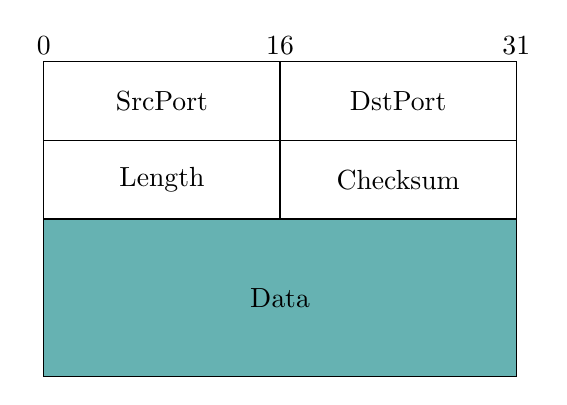
\begin{tikzpicture}
        \draw (0, 0) rectangle (3, -1);
        \draw (0, -1) rectangle (3, -2);
        \draw (3, 0) rectangle (6, -1);
        \draw (3, -1) rectangle (6, -2);
        \draw[fill=teal!60!white] (0, -2) rectangle (6, -4);

        \node at (1.5, -0.5) {SrcPort};
        \node at (4.5, -0.5) {DstPort};
        \node at (1.5, -1.5) {Length};
        \node at (4.5, -1.5) {Checksum};
        \node at (3, -3) {Data};

        \node at (0, 0.2) {0};
        \node at (3, 0.2) {16};
        \node at (6, 0.2) {31};
    \end{tikzpicture}
\end{figure}
\subsection{UDP Checksum}
\begin{itemize}[nosep]
    \item Uses the same algorithm as the IP checksum
          \begin{itemize}[nosep]
              \item Set checksum field to 0
              \item Sum all 16-bit words, adding any carry bits to the LSB
              \item Flip bits to get checksum (except $\texttt{0xffff}\to\texttt{0xffff}$)
              \item To check: sum whole packet, including sum, should get \texttt{0xffff}
          \end{itemize}
    \item How many errors?
          \begin{itemize}[nosep]
              \item Catches any 1-bit error
              \item Not all 2-bit errors
          \end{itemize}
    \item Optional in IPv4: not checked if value is 0
\end{itemize}
\subsection{Pseudo Header}
\begin{figure}[H]
    \begin{bytefield}{32}
        \bitheader{0,7,8,15,16,23,24,31}\\
        \wordbox{1}{source address}\\
        \wordbox{1}{destination address}\\
        \bitboxes{8}{{zero}{protocol}} & \bitbox{16}{UDP length}
    \end{bytefield}
\end{figure}
\begin{itemize}[nosep]
    \item UDP Checksum is computed over \emph{pseudo-header} prepended to the UDP header
          \begin{itemize}[nosep]
              \item For IPv4: IP Source, IP Dest, Protocol (=17), plus UDP length
          \end{itemize}
    \item Benefits? Problems?
          \begin{itemize}[nosep]
              \item Is UDP a layer on top of IP?
          \end{itemize}
\end{itemize}
\url{http://www.postel.org/pipermail/end2end-interest/2005-February/004616.html}

\subsection{Next Problem: Reliability}
\begin{table}[H]
    \begin{tabular}{ll}
        Problem               & Mechanism                   \\\toprule
        Dropped Packets       & Acknowledgements + Timeout  \\
        Duplicate Packets     & Sequene Numbers             \\
        Packets out of Order  & Receiver Window             \\
        Keeping the pipe full & Sliding Window (Pipelining)
    \end{tabular}
\end{table}

\subsection{Transport Layer Reliability}
\begin{itemize}[nosep]
    \item Extra difficulties
          \begin{itemize}[nosep]
              \item Multiple hosts
              \item Multiple hops
              \item Multiple potential paths
          \end{itemize}
    \item Need for connection establishments, tear down
          \begin{itemize}[nosep]
              \item Analogy: dialing a number versus a direct line
          \end{itemize}
    \item Varring RTTs
          \begin{itemize}[nosep]
              \item Both across connections and \emph{during} a connection
              \item Why do they vary? What do they influence?
          \end{itemize}
    \item Out of order packets
          \begin{itemize}[nosep]
              \item Not only because of drops/retransmissions
              \item Can get very old packets (up to 120s), must not get confused
          \end{itemize}
    \item Unknown resources at other end
          \begin{itemize}[nosep]
              \item Must be able to discover receiver buffer: flow control
          \end{itemize}
    \item Unknown resources in the network
          \begin{itemize}[nosep]
              \item Should not overload the network
              \item But should use as much as safely possible
              \item Congestion Control
          \end{itemize}
\end{itemize}
\subsection{TCP -- Transmission Control Protocol}
\begin{itemize}[nosep]
    \item Service model: ``reliable, connection oriented, full duplex byte stream''
          \begin{itemize}[nosep]
              \item Endpoints: <IP Address, Port>
          \end{itemize}
    \item Flow control
          \begin{itemize}[nosep]
              \item If one end stops reading, writes at other eventually stop/fail
          \end{itemize}
    \item Congestion control
          \begin{itemize}[nosep]
              \item Keeps sender from overloading the network
          \end{itemize}
\end{itemize}
\subsection{TCP}
\begin{itemize}[nosep]
    \item Specification
          \begin{itemize}[nosep]
              \item RFC 793 (1981), RFC 1222 (1989, some corrections), RFC 5681 (2009, congestion control), \dots
          \end{itemize}
    \item Was born coupled with IP, later factored out
    \item End-to-end protocol
          \begin{itemize}[nosep]
              \item Minimal assumptions on the network
              \item All mechanisms run on the end points
          \end{itemize}
    \item Alternative idea:
          \begin{itemize}[nosep]
              \item Provide reliability, flow control, etc, link-by-link
              \item Does it work?
          \end{itemize}
\end{itemize}
\subsection{TCP Header}
\begin{figure}[H]
    \begin{bytefield}[bitwidth=0.03\textwidth]{32}
        \bitheader{0-31}\\
        \bitboxes{16}{{Source Port}{Destination Port}}\\
        \wordbox{1}{Sequence Number}\\
        \wordbox{1}{Acknowledgement Number}\\
        \bitbox[lr]{4}{Data} & \bitbox[lr]{3}{} & \bitboxes[lr]{1}{NCWUAPRSF} & \bitbox[lr]{16}{}\\
        \bitbox[lr]{4}{Offset} & \bitbox[lr]{3}{Reserved} & \bitboxes[lr]{1}{SWCRCSSYI} & \bitbox[lr]{16}{Window}\\
        \bitbox[lr]{4}{} & \bitbox[lr]{3}{} & \bitboxes[lr]{1}{{}REGKHTNN} & \bitbox[lr]{16}{}\\
        \bitbox{24}{Options} & \bitbox{8}{Padding}\\
        \wordbox{1}{data}
    \end{bytefield}
\end{figure}
\subsection{Header Fields}
\begin{itemize}[nosep]
    \item Ports: multiplexing
    \item Sequence number
          \begin{itemize}[nosep]
              \item Correspond to \emph{bytes}, not packets!
          \end{itemize}
    \item Acknowledgement Number
          \begin{itemize}[nosep]
              \item Next expected sequence number
          \end{itemize}
    \item Window: willing to receive
          \begin{itemize}[nosep]
              \item Lets receiver limit SWS (even to 0) for flow control
          \end{itemize}
    \item Data Offset: number of 4 byte header + option bytes
    \item Flags, Checksum, Urgen Pointer
\end{itemize}
\subsection{Header Flags}
\begin{itemize}[nosep]
    \item URG: whether there is urgent data
    \item ACK: ack no. valid (all but first segment)
    \item PSH: push data to the application immediately
    \item RST: reset connection
    \item SYN: synchronize, establishes connection
    \item FIN: close connection
\end{itemize}

\subsection{Establishing a Connection}
\begin{itemize}[nosep]
    \item Three-way handshake
    \item Two sides agree on respective initial sequence nums
    \item If no one is listening on port: server sends RST
    \item If server is overloaded: ignore SYN
    \item If no SYN-ACK: retry, timeout
\end{itemize}

\subsection{Connection Termination}
\begin{itemize}[nosep]
    \item FIN bit says no more data to send
          \begin{itemize}[nosep]
              \item Caused by close or shutdown
              \item Both sides must send FIN to close a connection
          \end{itemize}
    \item Typical close
\end{itemize}

\subsection{TIME\_WAIT}
\begin{itemize}[nosep]
    \item Why do yo have to wait for 2MSL in TIME\_WAIT?
          \begin{itemize}[nosep]
              \item What if last ACK is severely delayed, \emph{and}
              \item Same port pair is immediately reused for a new connection?
          \end{itemize}
    \item Solution: active closer goes into TIME\_WAIT
          \begin{itemize}[nosep]
              \item Waits for 2MSL (Maximum Segment Lifetime)
          \end{itemize}
    \item Can be problematic for active servers
          \begin{itemize}[nosep]
              \item OS has too many sockets in TIME\_WAIT, can accept fewer connections
                    \begin{itemize}[nosep]
                        \item Hack: send RST and dlete socket, SO\_LINGER = 0
                    \end{itemize}
              \item OS won't let you restart server because port in use
                    \begin{itemize}[nosep]
                        \item SO\_REUSEADDR lets you rebind
                    \end{itemize}
          \end{itemize}
\end{itemize}

\subsection{Reliable Delivery}
\begin{itemize}[nosep]
    \item TCP retransmits if data corrupted or dropped
          \begin{itemize}[nosep]
              \item Also retransmit if ACK lost
          \end{itemize}
    \item When should TCP retransmit?
    \item Challenges in estimating RTT
          \begin{itemize}[nosep]
              \item Dynamic
              \item No additional traffic
          \end{itemize}
\end{itemize}

\subsection{Smoothing RTT}
\begin{itemize}[nosep]
    \item RTT measurement can have large variation
    \item Need to smooth the samples
          \begin{itemize}[nosep]
              \item One RTT measurement = one sample
          \end{itemize}
    \item Some ways to smooth the sample
          \begin{itemize}[nosep]
              \item Average of the whole sequence
              \item Windowed Mean
          \end{itemize}
    \item Problems?
\end{itemize}

\subsection{EWMA}
\begin{itemize}[nosep]
    \item EWMA: Exponentially Weighted Moving Average
    \item Give greater weight to recent samples.
          \begin{itemize}[nosep]
              \item Why?
          \end{itemize}
          \url{https://en.wikipedia.org/wiki/Moving_average#Exponential_moving_average}
    \item Estimate RTT
    \item $\textproc{RTT}(t) = \alpha \textproc{RTT}(t - 1) + (1 - \alpha) \texttt{newEst}$
    \item More generally, for a dataset $Y = Y_1, Y_2, \dots$
          \[S(t) = \begin{cases}Y_1 & t = 1\\\alpha Y_t + (1 - \alpha)S(t - 1) & t > 1\end{cases}\]
\end{itemize}